\documentclass{article}

\usepackage{fancyhdr}
\usepackage[margin=2cm]{geometry}
\usepackage{graphicx}
\usepackage{graphics}
\usepackage{hyperref}
\usepackage{psfrag}
\usepackage{ifthen}
\usepackage{array}
\usepackage{longtable}
\usepackage{color}
\usepackage{tikz}
\usetikzlibrary{arrows.meta}
\usepackage{bm}
\usepackage{amsmath, amsfonts}
\usepackage[shortlabels]{enumitem}
\setcounter{secnumdepth}{0}
\newcommand{\N}{\mathbb{N}}
\newcommand{\R}{\mathbb{R}}

\begin{document}

\title{Homework Set \#2}
\author{Hayden Pott (CWID: 103-99-9610)\\Worked With: Landen Nguyen}
\date{18 April 2024}

\fancyhead{}
\fancyhead[R]{Hayden Pott (CWID: 103-99-9610)}
\fancyhead[L]{Homework Set \#2}
\renewcommand\headrulewidth{0pt}
\fancyfoot{}
\fancyfoot[C]{\thepage}

\pagestyle{fancy}
\maketitle

\begin{enumerate}
\section{Lecture 5}
    \item Refer to Slide 4. True or False : The string ``abbabb" is a word
        in the language accepted by the transition graph? \\
        \textbf{ANSWER:} True

    \item Refer to Slide 5. How many SUCCESSFUL paths can the word ``abbabb"
        trace through this transition graph? \\
        \textbf{ANSWER:} 2

    \item Refer to Slide 9. How many TOTAL paths (successful and
        unsuccessful) can the word ``aabb" trace through the transition graph
        given near the bottom of the slide? \\
        \textbf{ANSWER:} 3

    \item Refer to Slide 11. True or False : This transition graph accepts
        every word that can be created from the alphabet $\{a, b\}$ that ends in
        ``aa"? \\
        \textbf{ANSWER:} True

    \item (Cohen, Chapter 6, Problem 19) A Student walks in to a class room
        and sees on the whiteboard a diagram of a TG with two states that
        accepts only the empty string, $\Lambda$. The student reverses the
        direction of exactly one edge, leaving all other edges and all labels
        and all +'s and -'s the same. But now the new TG accepts the language
        a*. What was the original machine? \\
        \textbf{ANSWER:}\\
        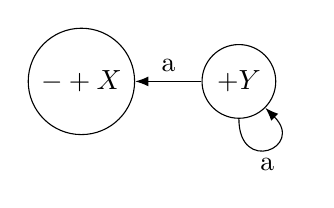
\begin{tikzpicture}[node distance={20mm}, main/.style = {draw, circle}]
            \node[main] (X) {$-+X$}; 
            \node[main] (Y) [right of=X] {$+Y$};

            \path[-Latex] (Y) edge node[above] {a} (X);

            \path[-Latex] (Y) edge [out=270,in=315,looseness=5] node[below] {a} (Y);
        \end{tikzpicture}

    \item Draw a transition graph (that is not also a finite automaton) to
        accept the Language($\bm{(a+b)*abb*}$) \\
        \textbf{ANSWER:}\\
        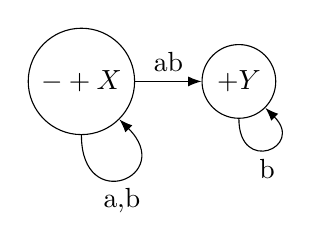
\begin{tikzpicture}[node distance={20mm}, main/.style = {draw, circle}]
            \node[main] (X) {$-+X$}; 
            \node[main] (Y) [right of=X] {$+Y$};

            \path[-Latex] (X) edge node[above] {ab} (Y);

            \path[-Latex] (Y) edge [out=270,in=315,looseness=5] node[below] {b} (Y);
            \path[-Latex] (X) edge [out=270,in=315,looseness=5] node[below] {a,b} (X);
        \end{tikzpicture}

\section{Lecture 6}

    \item True or False. Every transition graph is a finite automaton. \\
        \textbf{ANSWER}: False

    \item True or False. Transition graphs may have nodes with multiple outgoing arcs labeled 
    with the same letter -- e.g., two outgoing arcs labeled ``a" for instance. \\
        \textbf{ANSWER:} False

    \item True or False. Finite automata may have nodes with multiple incoming arcs labeled 
    with the same letter -- e.g., two incoming arcs labeled ``a" for instance. \\
        \textbf{ANSWER:} True
    
    \item Refer to Example 3 of the ``transition graph to regular expression" algorithm, 
    beginning on Slide 18. Solve this entire problem but delete State X before State Y. (I deleted 
    State Y before State X.) Show all steps. \\
        \textbf{ANSWER:} \\
        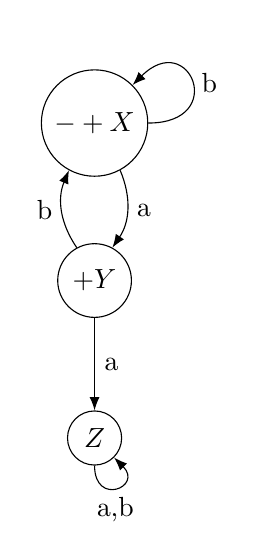
\begin{tikzpicture}[node distance={20mm}, main/.style = {draw, circle}]
            \node[main] (X) {$-+X$}; 
            \node[main] (Y) [below of=X] {$+Y$};
            \node[main] (Z) [below of=Y] {$Z$};

            \path[-Latex] (X) edge [out=0,in=45,looseness=5] node[right] {b} (X);

            \path[-Latex, bend left=10mm] (X) edge node[right] {a} (Y);
            \path[-Latex, bend left=10mm] (Y) edge node[left] {b} (X);

            \path[-Latex] (Y) edge node[right] {a} (Z);

            % \path[-Latex] (X) edge [out=270,in=315,looseness=5] node[below] {a,b} (X);
            \path[-Latex] (Z) edge [out=270,in=315,looseness=5] node[below] {a,b} (Z);
        \end{tikzpicture} \\
        Step 2.1 and 2.2 – Set up unique start and end states. \\
        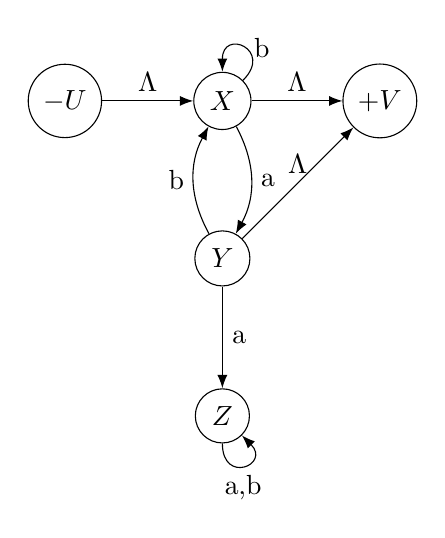
\begin{tikzpicture}[node distance={20mm}, main/.style = {draw, circle}]
            \node[main] (U) {$-U$};
            \node[main] (X) [right of=U]{$X$}; 
            \node[main] (Y) [below of=X] {$Y$};
            \node[main] (Z) [below of=Y] {$Z$};
            \node[main] (V) [right of=X] {$+V$};

            \path[-Latex] (X) edge [out=45,in=90,looseness=5] node[right] {b} (X);

            \path[-Latex, bend left=10mm] (X) edge node[right] {a} (Y);
            \path[-Latex, bend left=10mm] (Y) edge node[left] {b} (X);

            \path[-Latex] (Y) edge node[right] {a} (Z);

            \path[-Latex] (U) edge node[above] {$\Lambda$} (X);
            \path[-Latex] (X) edge node[above] {$\Lambda$} (V);
            \path[-Latex] (Y) edge node[above] {$\Lambda$} (V);

            % \path[-Latex] (X) edge [out=270,in=315,looseness=5] node[below] {a,b} (X);
            \path[-Latex] (Z) edge [out=270,in=315,looseness=5] node[below] {a,b} (Z);
        \end{tikzpicture} \\
        Step 2.3 and Step 2.4 – Not applicable \\
        Step 2.5 -- delete X \\
        Paths to preserve: \\
        \begin{itemize}
            \item $U \to V$
            \item $U \to Y$
            \item $Y \to V$
            \item $Y \to Y$
        \end{itemize}
        \begin{tikzpicture}[node distance={20mm}, main/.style = {draw, circle}]
            \node[main] (U) {$-U$};
            % \node[main] (X) [right of=U]{$X$}; 
            \node[main] (Y) [below of=X] {$Y$};
            \node[main] (Z) [below of=Y] {$Z$};
            \node[main] (V) [right of=X] {$+V$};

            % \path[-Latex] (X) edge [out=45,in=90,looseness=5] node[right] {b} (X);

            % \path[-Latex, bend left=10mm] (X) edge node[right] {a} (Y);
            % \path[-Latex, bend left=10mm] (Y) edge node[left] {b} (V);
            \path[-Latex] (Y) edge [out=270,in=315,looseness=5] node[right] {$\bm{bb*a}$} (Y);

            \path[-Latex] (Y) edge node[right] {a} (Z);

            \path[-Latex] (U) edge node[above] {$\bm{b^*}$} (V);
            \path[-Latex] (U) edge node[above] {$\bm{b^*a}$} (Y);
            \path[-Latex] (Y) edge node[above] {$\Lambda$, $\bm{bb^*}$} (V);

            % \path[-Latex] (X) edge [out=270,in=315,looseness=5] node[below] {a,b} (X);
            \path[-Latex] (Z) edge [out=270,in=315,looseness=5] node[below] {a,b} (Z);
        \end{tikzpicture} \\
        Step 2.3 - Combine $\Lambda$ and $\bm{bb*}$ into $\bm{\Lambda + bb*}$ \\
        \begin{tikzpicture}[node distance={20mm}, main/.style = {draw, circle}]
            \node[main] (U) {$-U$};
            % \node[main] (X) [right of=U]{$X$}; 
            \node[main] (Y) [below of=X] {$Y$};
            \node[main] (Z) [below of=Y] {$Z$};
            \node[main] (V) [right of=X] {$+V$};

            % \path[-Latex] (X) edge [out=45,in=90,looseness=5] node[right] {b} (X);

            % \path[-Latex, bend left=10mm] (X) edge node[right] {a} (Y);
            % \path[-Latex, bend left=10mm] (Y) edge node[left] {b} (V);

            \path[-Latex] (Y) edge node[right] {a} (Z);

            \path[-Latex] (U) edge node[above] {$\bm{b^*}$} (V);
            \path[-Latex] (U) edge node[above] {$\bm{b^*a}$} (Y);
            \path[-Latex] (Y) edge node[above] {$\bm{\Lambda + bb^*}$} (V);

            \path[-Latex] (Y) edge [out=270,in=315,looseness=5] node[right] {$\bm{bb^*a}$} (Y);
            \path[-Latex] (Z) edge [out=270,in=315,looseness=5] node[below] {a,b} (Z);
        \end{tikzpicture} \\

        Step 2.5 -- delete Y \\
        Paths to preserve: \\
        \begin{itemize}
            \item $U \to Z$
            \item $U \to V$
        \end{itemize}
        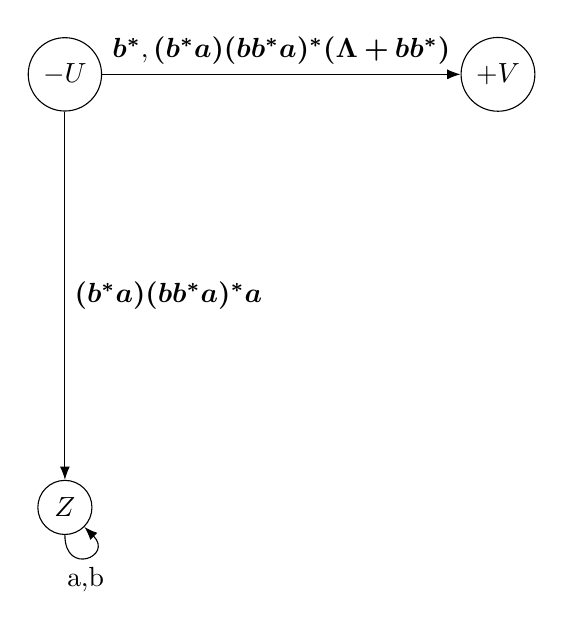
\begin{tikzpicture}[node distance={55mm}, main/.style = {draw, circle}]
            \node[main] (U) {$-U$};
            % \node[main] (X) [right of=U]{$X$}; 
            % \node[main] (Y) [below of=X] {$Y$};
            \node[main] (Z) [below of=U] {$Z$};
            \node[main] (V) [right of=U] {$+V$};

            % \path[-Latex] (X) edge [out=45,in=90,looseness=5] node[right] {b} (X);

            % \path[-Latex, bend left=10mm] (X) edge node[right] {a} (Y);
            % \path[-Latex, bend left=10mm] (Y) edge node[left] {b} (V);

            \path[-Latex] (U) edge node[above] {$\bm{b^*}, \bm{(b^*a)(bb^*a)^*(\Lambda + bb^*)}$} (V);
            \path[-Latex] (U) edge node[right] {$\bm{(b^*a)(bb^*a)^*a}$} (Z);

            \path[-Latex] (Z) edge [out=270,in=315,looseness=5] node[below] {a,b} (Z);
        \end{tikzpicture} \\
        Step 2.3 - Combine $\bm{b^*}$, $\bm{(b^*a)(bb^*a)^*(\Lambda + bb^*)}$ into $\bm{b^*} + \bm{(b^*a)(bb^*a)^*(\Lambda + bb^*)}$ \\
        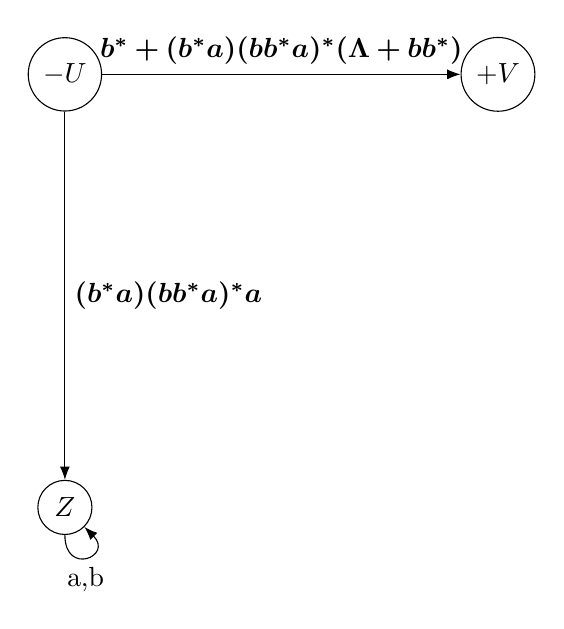
\begin{tikzpicture}[node distance={55mm}, main/.style = {draw, circle}]
            \node[main] (U) {$-U$};
            % \node[main] (X) [right of=U]{$X$}; 
            % \node[main] (Y) [below of=X] {$Y$};
            \node[main] (Z) [below of=U] {$Z$};
            \node[main] (V) [right of=U] {$+V$};

            % \path[-Latex] (X) edge [out=45,in=90,looseness=5] node[right] {b} (X);

            % \path[-Latex, bend left=10mm] (X) edge node[right] {a} (Y);
            % \path[-Latex, bend left=10mm] (Y) edge node[left] {b} (V);

            \path[-Latex] (U) edge node[above] {$\bm{b^* + (b^*a)(bb^*a)^*(\Lambda + bb^*)}$} (V);
            \path[-Latex] (U) edge node[right] {$\bm{(b^*a)(bb^*a)^*a}$} (Z);

            \path[-Latex] (Z) edge [out=270,in=315,looseness=5] node[below] {a,b} (Z);
        \end{tikzpicture} \\
        Thus, our final regular expression is $\bm{b^* + (b^*a)(bb^*a)^*(\Lambda + bb^*)}$.


    \item Refer to Example 4 of the ``transition graph to regular expression"
        algorithm, beginning on Slide 22. Solve this entire problem but delete
        State W, then State Y, then State Z. (I deleted states in the order Z,
        Y, W.) \\
        \textbf{ANSWER:} \\
        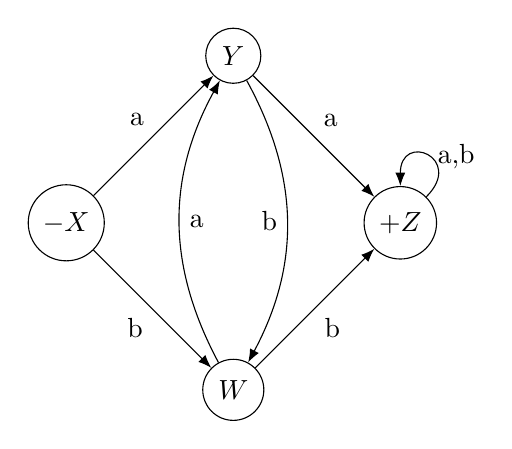
\begin{tikzpicture}[node distance={30mm}, main/.style = {draw, circle}]
            \node[main] (X) {$-X$};
            \node[main] (Y) [above right of=X] {$Y$};
            \node[main] (W) [below right of=X] {$W$};
            \node[main] (Z) [above right of=W] {$+Z$};

            \path[-Latex] (Z) edge [out=45,in=90,looseness=5] node[right] {a,b} (Z);
            \path[-Latex] (X) edge node[above left] {a} (Y);
            \path[-Latex] (X) edge node[below left] {b} (W);
            \path[-Latex] (W) edge node[below right] {b} (Z);
            \path[-Latex] (Y) edge node[above right] {a} (Z);

            \path[-Latex, bend left=10mm] (W) edge node[right] {a} (Y);
            \path[-Latex, bend left=10mm] (Y) edge node[left] {b} (W);
        \end{tikzpicture} \\
        Step 2.1 -- Not applicable \\
        Step 2.2 -- Add new end state \\
        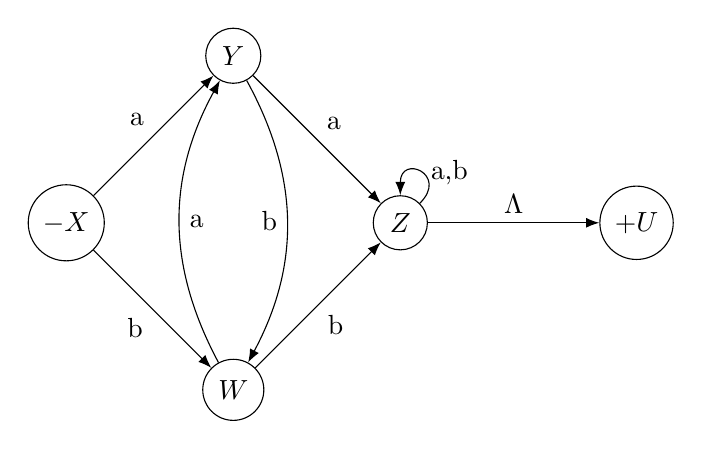
\begin{tikzpicture}[node distance={30mm}, main/.style = {draw, circle}]
            \node[main] (X) {$-X$};
            \node[main] (Y) [above right of=X] {$Y$};
            \node[main] (W) [below right of=X] {$W$};
            \node[main] (Z) [above right of=W] {$Z$};
            \node[main] (U) [right of=Z] {$+U$};

            \path[-Latex] (Z) edge [out=45,in=90,looseness=5] node[right] {a,b} (Z);
            \path[-Latex] (X) edge node[above left] {a} (Y);
            \path[-Latex] (X) edge node[below left] {b} (W);
            \path[-Latex] (W) edge node[below right] {b} (Z);
            \path[-Latex] (Y) edge node[above right] {a} (Z);

            \path[-Latex, bend left=10mm] (W) edge node[right] {a} (Y);
            \path[-Latex, bend left=10mm] (Y) edge node[left] {b} (W);

            \path[-Latex] (Z) edge node[above] {$\Lambda$} (U);
        \end{tikzpicture} \\
        Step 2.3 -- Combine a,b on $Z$\\
        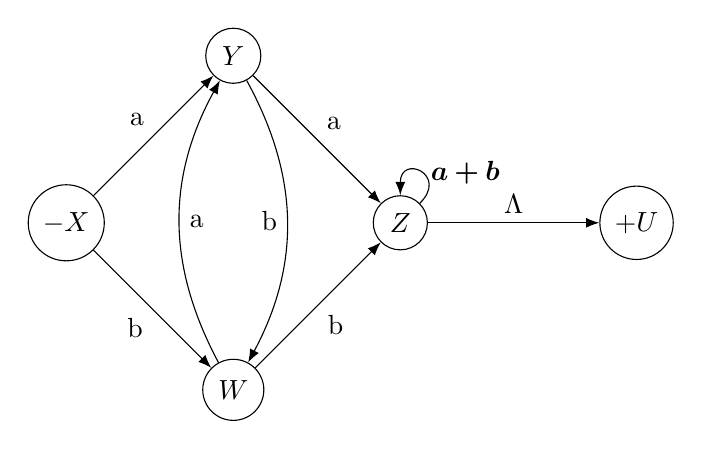
\begin{tikzpicture}[node distance={30mm}, main/.style = {draw, circle}]
            \node[main] (X) {$-X$};
            \node[main] (Y) [above right of=X] {$Y$};
            \node[main] (W) [below right of=X] {$W$};
            \node[main] (Z) [above right of=W] {$Z$};
            \node[main] (U) [right of=Z] {$+U$};

            \path[-Latex] (Z) edge [out=45,in=90,looseness=5] node[right] {$\bm{a + b}$} (Z);
            \path[-Latex] (X) edge node[above left] {a} (Y);
            \path[-Latex] (X) edge node[below left] {b} (W);
            \path[-Latex] (W) edge node[below right] {b} (Z);
            \path[-Latex] (Y) edge node[above right] {a} (Z);

            \path[-Latex, bend left=10mm] (W) edge node[right] {a} (Y);
            \path[-Latex, bend left=10mm] (Y) edge node[left] {b} (W);

            \path[-Latex] (Z) edge node[above] {$\Lambda$} (U);
        \end{tikzpicture} \\
        Step 2.4 -- Not applicable \\
        Step 2.5 -- Delete $W$ \\
        Paths to preserve: \\
        \begin{itemize}
            \item $X \to Y = \bm{ba}$
            \item $X \to Z = \bm{bb}$
            \item $Y \to Y = \bm{ba}$
            \item $Y \to Z = \bm{bb}$
        \end{itemize}
        \begin{tikzpicture}[node distance={30mm}, main/.style = {draw, circle}]
            \node[main] (X) {$-X$};
            \node[main] (Y) [above right of=X] {$Y$};
            % \node[main] (W) [below right of=X] {$W$};
            \node[main] (Z) [above right of=W] {$Z$};
            \node[main] (U) [right of=Z] {$+U$};

            \path[-Latex] (Z) edge [out=45,in=90,looseness=5] node[right] {$\bm{a + b}$} (Z);
            \path[-Latex] (Y) edge [out=45,in=90,looseness=5] node[right] {$\bm{ba}$} (Y);
            \path[-Latex] (X) edge node[above left] {a,$\bm{ba}$} (Y);
            \path[-Latex] (Y) edge node[above right] {a,$\bm{bb}$} (Z);
            \path[-Latex] (X) edge node[above right] {$\bm{bb}$} (Z);

            \path[-Latex] (Z) edge node[above] {$\Lambda$} (U);
        \end{tikzpicture} \\
        Step 2.3 -- Combine $X \to Y$ and $Y \to Z$ \\
        \begin{tikzpicture}[node distance={30mm}, main/.style = {draw, circle}]
            \node[main] (X) {$-X$};
            \node[main] (Y) [above right of=X] {$Y$};
            % \node[main] (W) [below right of=X] {$W$};
            \node[main] (Z) [above right of=W] {$Z$};
            \node[main] (U) [right of=Z] {$+U$};

            \path[-Latex] (Z) edge [out=45,in=90,looseness=5] node[right] {$\bm{a + b}$} (Z);
            \path[-Latex] (Y) edge [out=45,in=90,looseness=5] node[right] {$\bm{ba}$} (Y);
            \path[-Latex] (X) edge node[above left] {$\bm{a + ba}$} (Y);
            \path[-Latex] (Y) edge node[above right] {$\bm{a + bb}$} (Z);
            \path[-Latex] (X) edge node[above right] {$\bm{bb}$} (Z);

            \path[-Latex] (Z) edge node[above] {$\Lambda$} (U);
        \end{tikzpicture} \\
        Step 2.5 -- Delete $Y$ \\
        Paths to preserve: \\
        \begin{itemize}
            \item $X \to Z = \bm{(a + ba)(ba)^*(a+bb)}$
        \end{itemize}
        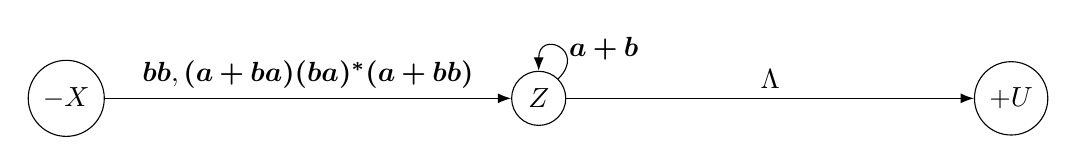
\begin{tikzpicture}[node distance={60mm}, main/.style = {draw, circle}]
            \node[main] (X) {$-X$};
            \node[main] (Z) [right of=X] {$Z$};
            \node[main] (U) [right of=Z] {$+U$};

            \path[-Latex] (Z) edge [out=45,in=90,looseness=5] node[right] {$\bm{a + b}$} (Z);
            \path[-Latex] (X) edge node[above] {$\bm{bb},\bm{(a + ba)(ba)^*(a+bb)}$} (Z);

            \path[-Latex] (Z) edge node[above] {$\Lambda$} (U);
        \end{tikzpicture} \\
        Step 2.3 -- Combine $X \to Z$ \\
        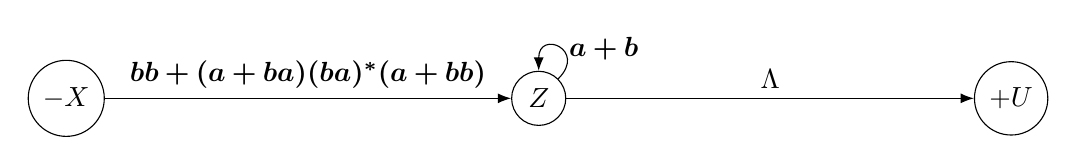
\begin{tikzpicture}[node distance={60mm}, main/.style = {draw, circle}]
            \node[main] (X) {$-X$};
            \node[main] (Z) [right of=X] {$Z$};
            \node[main] (U) [right of=Z] {$+U$};

            \path[-Latex] (Z) edge [out=45,in=90,looseness=5] node[right] {$\bm{a + b}$} (Z);
            \path[-Latex] (X) edge node[above] {$\bm{bb + (a + ba)(ba)^*(a+bb)}$} (Z);

            \path[-Latex] (Z) edge node[above] {$\Lambda$} (U);
        \end{tikzpicture} \\
        Step 2.5 -- Delete $Z$ \\
        Preserve Paths: \\
        \begin{itemize}
            \item $X \to U = \bm{(bb + (a + ba)(ba)^*(a+bb))(a + b)^*}$
        \end{itemize}
        \begin{tikzpicture}[node distance={60mm}, main/.style = {draw, circle}]
            \node[main] (X) {$-X$};
            % \node[main] (Z) [right of=X] {$Z$};
            \node[main] (U) [right of=Z] {$+U$};

            % \path[-Latex] (Z) edge [out=45,in=90,looseness=5] node[right] {$\bm{a + b}$} (Z);
            % \path[-Latex] (X) edge node[above] {$\bm{bb + (a + ba)(ba)^*(a+bb)}$} (Z);
            \path[-Latex] (X) edge node[above] {$\bm{(bb + (a + ba)(ba)^*(a+bb))(a + b)^*}$} (U);
        \end{tikzpicture} \\
        Thus, our final regular expression is $\bm{(bb + (a + ba)(ba)^*(a+bb))(a + b)^*}$.

\section{Lecture 7}

    \item Construct finite automata for the regular expressions: $\bm{a}$, $\bm{b}$, and 
        $\bm{\Lambda}$ using the algorithm given in part 3.1 of the proof of Kleene's Theorem. \\
        \textbf{ANSWER:} \\
        For $\bm{a}$: \\
        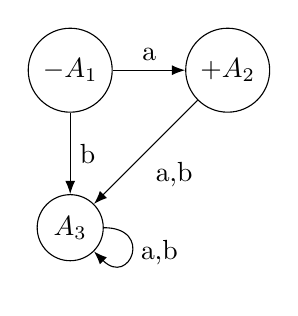
\begin{tikzpicture}[node distance={20mm}, main/.style = {draw, circle}]
            \node[main] (X) {$-A_1$};
            \node[main] (Y) [right of=X] {$+A_2$};
            \node[main] (Z) [below of=X] {$A_3$};

            \path[-Latex] (X) edge node[above] {a} (Y);
            \path[-Latex] (X) edge node[right] {b} (Z);
            \path[-Latex] (Y) edge node[below right] {a,b} (Z);

            \path[-Latex] (Z) edge [out=0,in=-45,looseness=5] node[right] {a,b} (Z);
        \end{tikzpicture} \\
        For $\bm{b}$: \\
        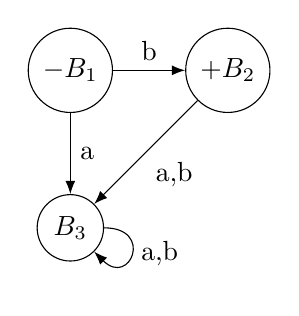
\begin{tikzpicture}[node distance={20mm}, main/.style = {draw, circle}]
            \node[main] (X) {$-B_1$};
            \node[main] (Y) [right of=X] {$+B_2$};
            \node[main] (Z) [below of=X] {$B_3$};

            \path[-Latex] (X) edge node[above] {b} (Y);
            \path[-Latex] (X) edge node[right] {a} (Z);
            \path[-Latex] (Y) edge node[below right] {a,b} (Z);

            \path[-Latex] (Z) edge [out=0,in=-45,looseness=5] node[right] {a,b} (Z);
        \end{tikzpicture} \\
        For $\bm{\Lambda}$: \\
        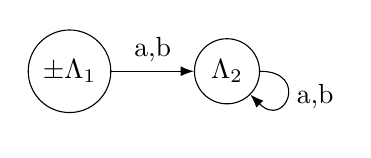
\begin{tikzpicture}[node distance={20mm}, main/.style = {draw, circle}]
            \node[main] (X) {$\pm\Lambda_1$};
            \node[main] (Y) [right of=X] {$\Lambda_2$};

            \path[-Latex] (X) edge node[above] {a,b} (Y);
            \path[-Latex] (Y) edge [out=0,in=-45,looseness=5] node[right] {a,b} (Y);
        \end{tikzpicture}

    \item Construct a finite automaton for the regular expression: $\bm{a + \Lambda}$
        using the algorithm given in part 3.2 of the proof of Kleene's Theorem.
        \\
        \textbf{ANSWER:} \\
        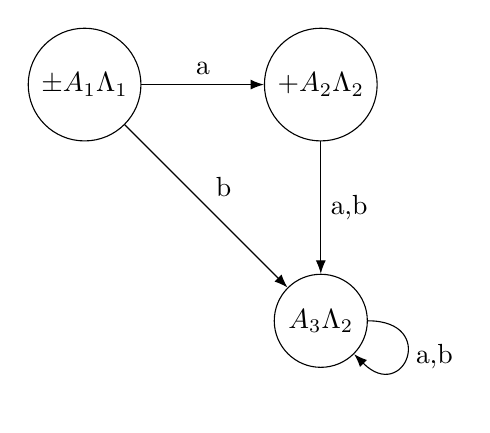
\begin{tikzpicture}[node distance={30mm}, main/.style = {draw, circle}]
            \node[main] (A1L1) {$\pm A_1\Lambda_1$};
            \node[main] (A2L2) [right of=A1L1] {$+A_2\Lambda_2$};
            \node[main] (A3L2) [below of=A2L2] {$A_3\Lambda_2$};

            \path[-Latex] (A1L1) edge node[above] {a} (A2L2);
            \path[-Latex] (A1L1) edge node[above right] {b} (A3L2);
            \path[-Latex] (A3L2) edge [out=0,in=-45,looseness=5] node[right] {a,b} (A3L2);
            \path[-Latex] (A2L2) edge node[right] {a,b} (A3L2);
        \end{tikzpicture}
        \newpage

    \item Construct a finite automaton for the regular expression: $\bm{b^*}$ using the 
        algorithm given in part 3.4 of the proof of Kleene's Theorem. \\
        \textbf{ANSWER:} \\
        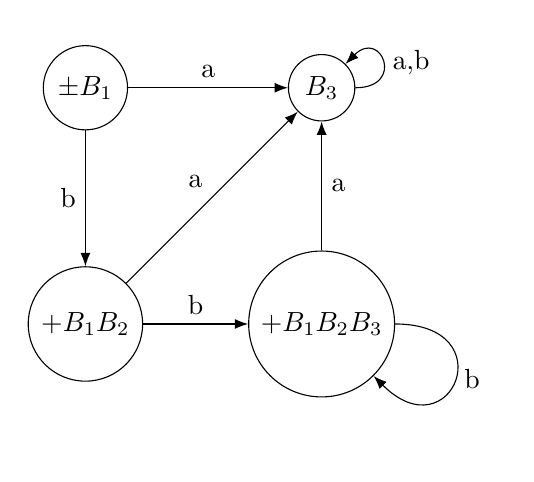
\begin{tikzpicture}[node distance={30mm}, main/.style = {draw, circle}]
            \node[main] (B1) {$\pm B_1$};
            \node[main] (B1B2) [below of=B1] {$+B_1B_2$};
            \node[main] (B3) [right of=B1] {$B_3$};
            \node[main] (B1B2B3) [below of=B3] {$+B_1B_2B_3$};

            \path[-Latex] (B1) edge node[left] {b} (B1B2);
            \path[-Latex] (B1B2) edge node[above] {b} (B1B2B3);
            \path[-Latex] (B1) edge node[above] {a} (B3);
            \path[-Latex] (B1B2B3) edge node[right] {a} (B3);
            \path[-Latex] (B1B2) edge node[above left] {a} (B3);

            \path[-Latex] (B1B2B3) edge [out=0,in=-45,looseness=5] node[right] {b} (B1B2B3);
            \path[-Latex] (B3) edge [out=0,in=45,looseness=5] node[right] {a,b} (B3);

        \end{tikzpicture}

    \item Construct finite automata for the regular expressions: $\bm{(a + 
        \Lambda)b*}$ using the algorithm given in part 3.3 of the proof of Kleene's 
        Theorem. \\
        \textbf{ANSWER:} \\
        $\bm{(a + \Lambda)}$: \\
        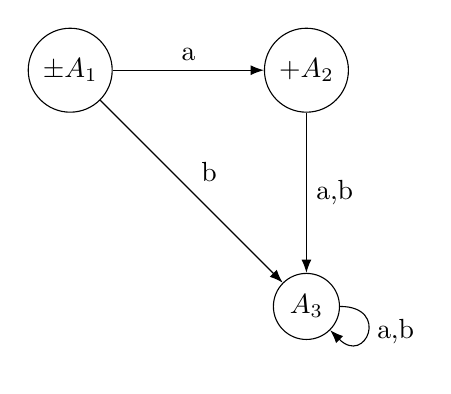
\begin{tikzpicture}[node distance={30mm}, main/.style = {draw, circle}]
            \node[main] (A1) {$\pm A_1$};
            \node[main] (A2) [right of=A1] {$+A_2$};
            \node[main] (A3) [below of=A2] {$A_3$};

            \path[-Latex] (A1) edge node[above] {a} (A2);
            \path[-Latex] (A1) edge node[above right] {b} (A3);
            \path[-Latex] (A3) edge [out=0,in=-45,looseness=5] node[right] {a,b} (A3);
            \path[-Latex] (A2) edge node[right] {a,b} (A3);
        \end{tikzpicture} \\
        $\bm{(b^*)}$: \\
        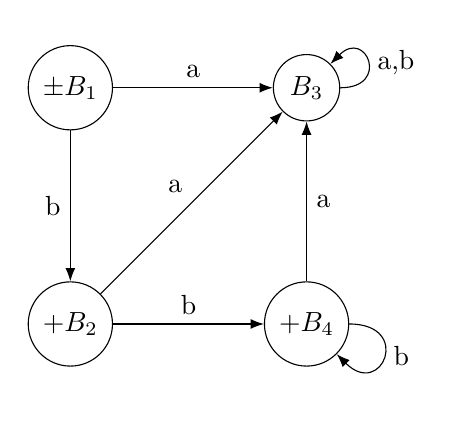
\begin{tikzpicture}[node distance={30mm}, main/.style = {draw, circle}]
            \node[main] (B1) {$\pm B_1$};
            \node[main] (B2) [below of=B1] {$+B_2$};
            \node[main] (B3) [right of=B1] {$B_3$};
            \node[main] (B4) [below of=B3] {$+B_4$};

            \path[-Latex] (B1) edge node[left] {b} (B2);
            \path[-Latex] (B2) edge node[above] {b} (B4);
            \path[-Latex] (B1) edge node[above] {a} (B3);
            \path[-Latex] (B4) edge node[right] {a} (B3);
            \path[-Latex] (B2) edge node[above left] {a} (B3);

            \path[-Latex] (B4) edge [out=0,in=-45,looseness=5] node[right] {b} (B4);
            \path[-Latex] (B3) edge [out=0,in=45,looseness=5] node[right] {a,b} (B3);
        \end{tikzpicture} \\

        \textbf{Step 1}: Create the starting state, $A_1B_1$ which contains $B_1$ because
        $A_1$ is accepting and is accepting because $B_1$ is accepting. \\
        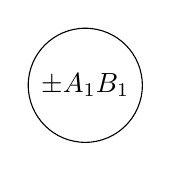
\begin{tikzpicture}[node distance={30mm}, main/.style = {draw, circle}]
            \node[main] (A1B1) {$\pm A_1B_1$};
        \end{tikzpicture}

        \textbf{Step 2}: From the starting state, follow the paths for a and b,
        which creates two new states, $A_2B_1B_3$ (accepting because $B_1$ is
        accepting) and $A_3B_2$ (accepting because $B_1$ is accepting). \\
        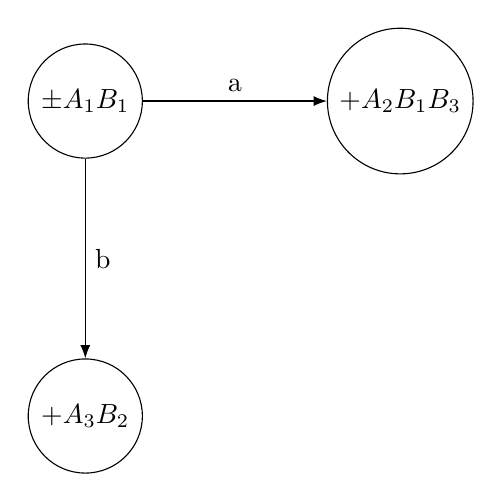
\begin{tikzpicture}[node distance={40mm}, main/.style = {draw, circle}]
            \node[main] (A1B1) {$\pm A_1B_1$};
            
            \node[main] (A2B1B3) [right of=A1B1] {$+ A_2B_1B_3$};
            \node[main] (A3B2) [below of=A1B1] {$+ A_3B_2$};

            \path[-Latex] (A1B1) edge node[above] {a} (A2B1B3);
            \path[-Latex] (A1B1) edge node[right] {b} (A3B2);
        \end{tikzpicture}

        \textbf{Step 2}: From the $A_2B_1B_3$ state, follow the paths for a and b,
        which creates two new states, $A_3B_3$ and $A_3B_2B_3$ (accepting because $B_2$ is accepting). \\
        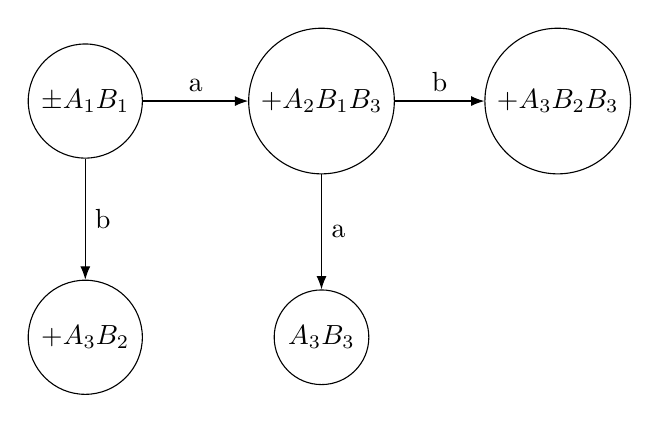
\begin{tikzpicture}[node distance={30mm}, main/.style = {draw, circle}]
            \node[main] (A1B1) {$\pm A_1B_1$};

            \node[main] (A2B1B3) [right of=A1B1] {$+ A_2B_1B_3$};
            \node[main] (A3B2) [below of=A1B1] {$+ A_3B_2$};

            \path[-Latex] (A1B1) edge node[above] {a} (A2B1B3);
            \path[-Latex] (A1B1) edge node[right] {b} (A3B2);

            \node[main] (A3B3) [below of=A2B1B3] {$A_3B_3$};
            \node[main] (A3B2B3) [right of=A2B1B3] {$+ A_3B_2B_3$};

            \path[-Latex] (A2B1B3) edge node[right] {a} (A3B3);
            \path[-Latex] (A2B1B3) edge node[above] {b} (A3B2B3);
        \end{tikzpicture}

        \textbf{Step 3}: From the $A_3B_2$ state, follow the paths for a and b,
        which creates one new state, $A_3B_4$ (accepting because $B_4$ is
        accepting) and links to $A_3B_3$. \\
        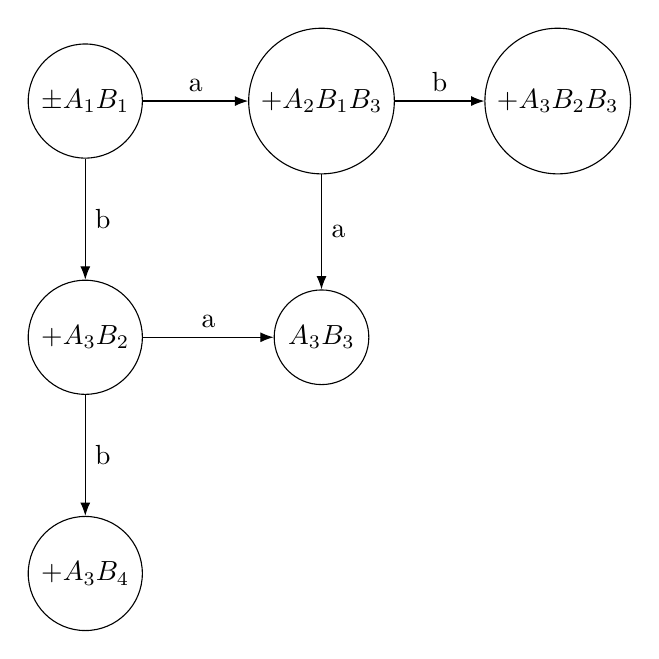
\begin{tikzpicture}[node distance={30mm}, main/.style = {draw, circle}]
            \node[main] (A1B1) {$\pm A_1B_1$};

            \node[main] (A2B1B3) [right of=A1B1] {$+ A_2B_1B_3$};
            \node[main] (A3B2) [below of=A1B1] {$+ A_3B_2$};

            \path[-Latex] (A1B1) edge node[above] {a} (A2B1B3);
            \path[-Latex] (A1B1) edge node[right] {b} (A3B2);

            \node[main] (A3B3) [below of=A2B1B3] {$A_3B_3$};
            \node[main] (A3B2B3) [right of=A2B1B3] {$+ A_3B_2B_3$};

            \path[-Latex] (A2B1B3) edge node[right] {a} (A3B3);
            \path[-Latex] (A2B1B3) edge node[above] {b} (A3B2B3);

            \node[main] (A3B4) [below of=A3B2] {$+ A_3B_4$};

            \path[-Latex] (A3B2) edge node[right] {b} (A3B4);
            \path[-Latex] (A3B2) edge node[above] {a} (A3B3);
        \end{tikzpicture}

        \textbf{Step 4}: From the $A_3B_4$ state, follow the paths for a and b,
        which links to $A_3B_3$ and loops to itself. \\
        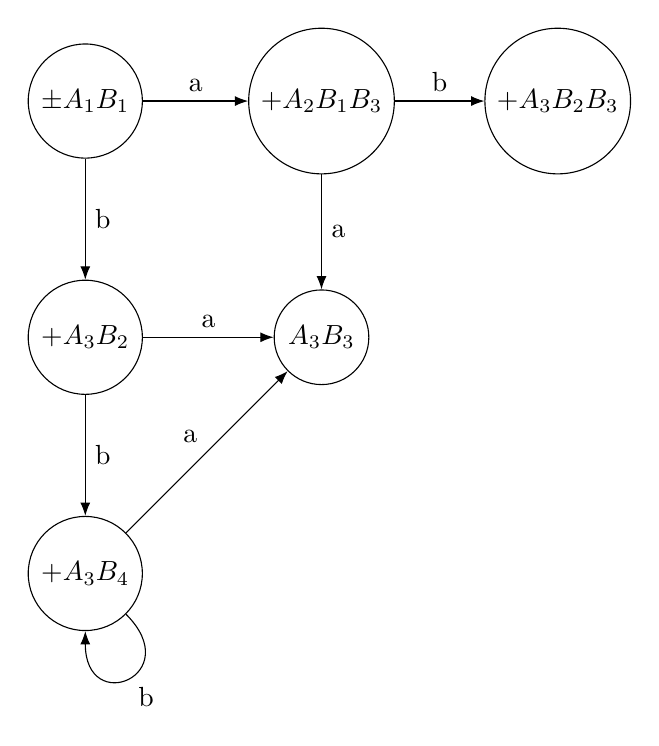
\begin{tikzpicture}[node distance={30mm}, main/.style = {draw, circle}]
            \node[main] (A1B1) {$\pm A_1B_1$};

            \node[main] (A2B1B3) [right of=A1B1] {$+ A_2B_1B_3$};
            \node[main] (A3B2) [below of=A1B1] {$+ A_3B_2$};

            \path[-Latex] (A1B1) edge node[above] {a} (A2B1B3);
            \path[-Latex] (A1B1) edge node[right] {b} (A3B2);

            \node[main] (A3B3) [below of=A2B1B3] {$A_3B_3$};
            \node[main] (A3B2B3) [right of=A2B1B3] {$+ A_3B_2B_3$};

            \path[-Latex] (A2B1B3) edge node[right] {a} (A3B3);
            \path[-Latex] (A2B1B3) edge node[above] {b} (A3B2B3);

            \node[main] (A3B4) [below of=A3B2] {$+ A_3B_4$};

            \path[-Latex] (A3B2) edge node[right] {b} (A3B4);
            \path[-Latex] (A3B2) edge node[above] {a} (A3B3);

            \path[-Latex] (A3B4) edge node[above left] {a} (A3B3);
            \path[-Latex] (A3B4) edge [out=-45,in=-90,looseness=5] node[below right] {b} (A3B4);
        \end{tikzpicture}

        \textbf{Step 5}: From the $A_3B_3$ state, follow the paths for a and b,
        which loops to itself. \\
        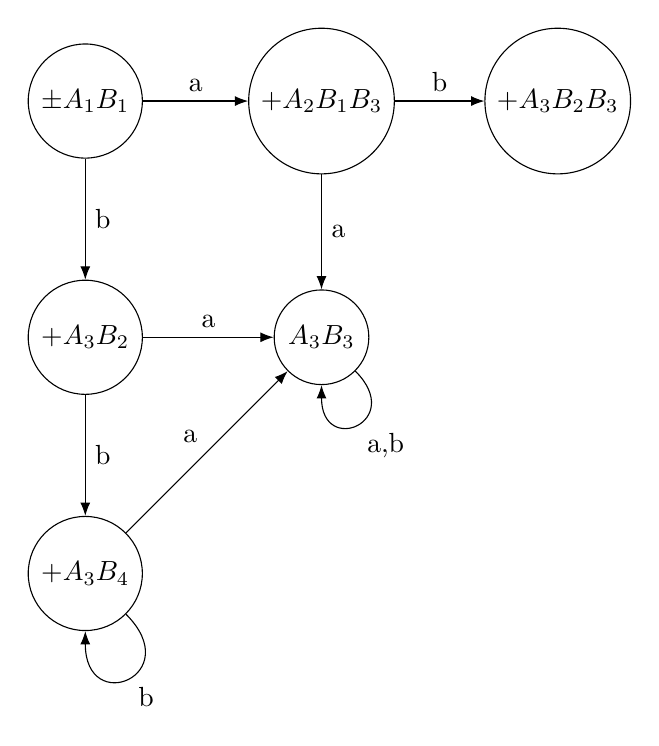
\begin{tikzpicture}[node distance={30mm}, main/.style = {draw, circle}]
            \node[main] (A1B1) {$\pm A_1B_1$};

            \node[main] (A2B1B3) [right of=A1B1] {$+ A_2B_1B_3$};
            \node[main] (A3B2) [below of=A1B1] {$+ A_3B_2$};

            \path[-Latex] (A1B1) edge node[above] {a} (A2B1B3);
            \path[-Latex] (A1B1) edge node[right] {b} (A3B2);

            \node[main] (A3B3) [below of=A2B1B3] {$A_3B_3$};
            \node[main] (A3B2B3) [right of=A2B1B3] {$+ A_3B_2B_3$};

            \path[-Latex] (A2B1B3) edge node[right] {a} (A3B3);
            \path[-Latex] (A2B1B3) edge node[above] {b} (A3B2B3);

            \node[main] (A3B4) [below of=A3B2] {$+ A_3B_4$};

            \path[-Latex] (A3B2) edge node[right] {b} (A3B4);
            \path[-Latex] (A3B2) edge node[above] {a} (A3B3);

            \path[-Latex] (A3B4) edge node[above left] {a} (A3B3);
            \path[-Latex] (A3B4) edge [out=-45,in=-90,looseness=5] node[below right] {b} (A3B4);

            \path[-Latex] (A3B3) edge [out=-45,in=-90,looseness=5] node[below right] {a,b} (A3B3);
        \end{tikzpicture}

        \textbf{Step 6}: From the $A_3B_2B_3$ state, follow the paths for a and b,
        which creates a new state, $A_3B_4B_3$ (accepting because $B_4$ is
        accepting and links to $A_3B_3$. \\
        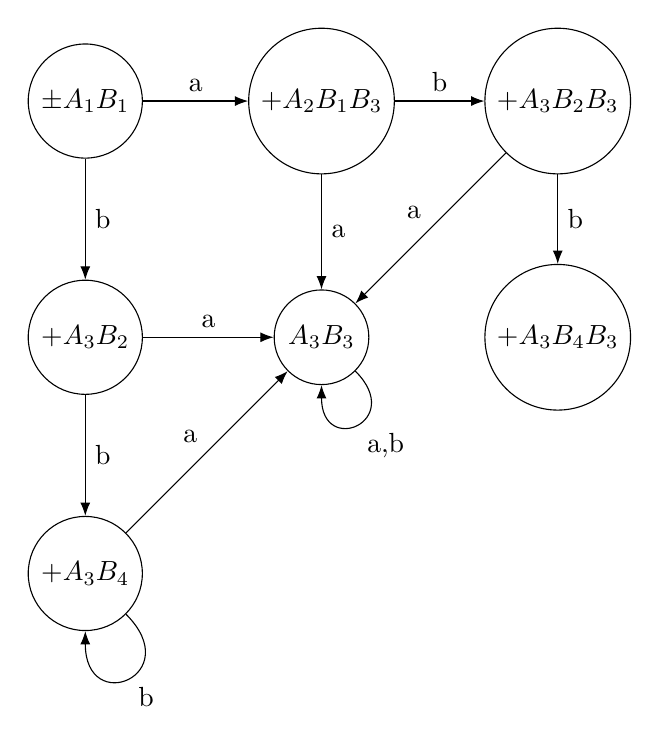
\begin{tikzpicture}[node distance={30mm}, main/.style = {draw, circle}]
            \node[main] (A1B1) {$\pm A_1B_1$};

            \node[main] (A2B1B3) [right of=A1B1] {$+ A_2B_1B_3$};
            \node[main] (A3B2) [below of=A1B1] {$+ A_3B_2$};

            \path[-Latex] (A1B1) edge node[above] {a} (A2B1B3);
            \path[-Latex] (A1B1) edge node[right] {b} (A3B2);

            \node[main] (A3B3) [below of=A2B1B3] {$A_3B_3$};
            \node[main] (A3B2B3) [right of=A2B1B3] {$+ A_3B_2B_3$};

            \path[-Latex] (A2B1B3) edge node[right] {a} (A3B3);
            \path[-Latex] (A2B1B3) edge node[above] {b} (A3B2B3);

            \node[main] (A3B4) [below of=A3B2] {$+ A_3B_4$};

            \path[-Latex] (A3B2) edge node[right] {b} (A3B4);
            \path[-Latex] (A3B2) edge node[above] {a} (A3B3);

            \path[-Latex] (A3B4) edge node[above left] {a} (A3B3);
            \path[-Latex] (A3B4) edge [out=-45,in=-90,looseness=5] node[below right] {b} (A3B4);

            \path[-Latex] (A3B3) edge [out=-45,in=-90,looseness=5] node[below right] {a,b} (A3B3);

            \node[main] (A3B4B3) [below of=A3B2B3] {$+ A_3B_4B_3$};

            \path[-Latex] (A3B2B3) edge node[right] {b} (A3B4B3);
            \path[-Latex] (A3B2B3) edge node[above left] {a} (A3B3);
        \end{tikzpicture}

        \textbf{Step 7}: From the $A_3B_4B_3$ state, follow the paths for a and b,
        which link to $A_3B_3$ and loop on itself. \\
        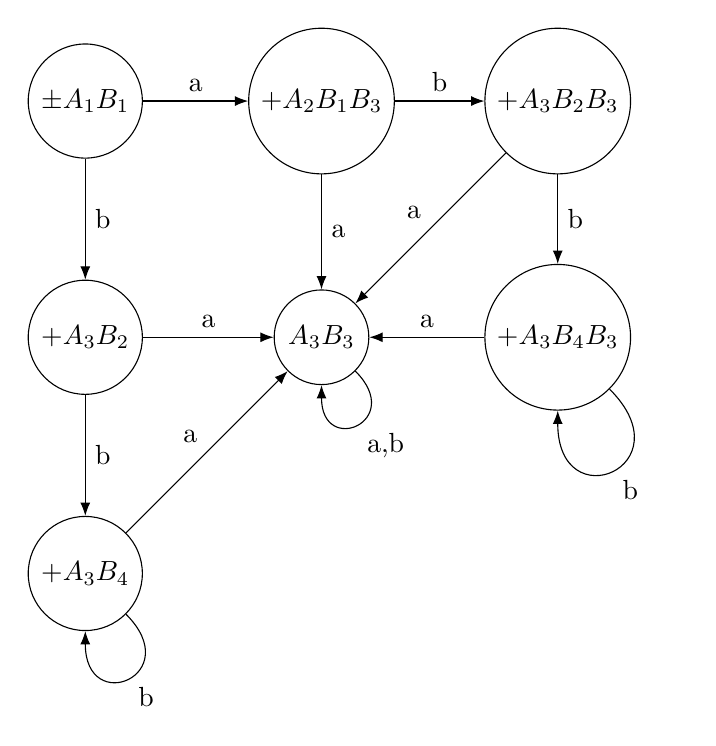
\begin{tikzpicture}[node distance={30mm}, main/.style = {draw, circle}]
            \node[main] (A1B1) {$\pm A_1B_1$};

            \node[main] (A2B1B3) [right of=A1B1] {$+ A_2B_1B_3$};
            \node[main] (A3B2) [below of=A1B1] {$+ A_3B_2$};

            \path[-Latex] (A1B1) edge node[above] {a} (A2B1B3);
            \path[-Latex] (A1B1) edge node[right] {b} (A3B2);

            \node[main] (A3B3) [below of=A2B1B3] {$A_3B_3$};
            \node[main] (A3B2B3) [right of=A2B1B3] {$+ A_3B_2B_3$};

            \path[-Latex] (A2B1B3) edge node[right] {a} (A3B3);
            \path[-Latex] (A2B1B3) edge node[above] {b} (A3B2B3);

            \node[main] (A3B4) [below of=A3B2] {$+ A_3B_4$};

            \path[-Latex] (A3B2) edge node[right] {b} (A3B4);
            \path[-Latex] (A3B2) edge node[above] {a} (A3B3);

            \path[-Latex] (A3B4) edge node[above left] {a} (A3B3);
            \path[-Latex] (A3B4) edge [out=-45,in=-90,looseness=5] node[below right] {b} (A3B4);

            \path[-Latex] (A3B3) edge [out=-45,in=-90,looseness=5] node[below right] {a,b} (A3B3);

            \node[main] (A3B4B3) [below of=A3B2B3] {$+ A_3B_4B_3$};

            \path[-Latex] (A3B2B3) edge node[right] {b} (A3B4B3);
            \path[-Latex] (A3B2B3) edge node[above left] {a} (A3B3);

            \path[-Latex] (A3B4B3) edge node[above] {a} (A3B3);
            \path[-Latex] (A3B4B3) edge [out=-45,in=-90,looseness=5] node[below right] {b} (A3B4B3);
        \end{tikzpicture}


\section{Lecture 8}

    \item (True or False) Non-deterministic Finite Automata (NFA) may have
        strings of characters on their arcs. \\
        \textbf{ANSWER:} False

    \item (True or False) Non-deterministic Finite Automata (NFA) may have
        and incoming arc from each state for each letter of the alphabet. \\
        \textbf{ANSWER:} True

    \item (True or False) The algorithm provided for constructing a finite
        automaton (FA) for the \underline{complement} of a regular language will
        ALWAYS generate a finite automaton for some regular language. \\
        \textbf{ANSWER:} True

    \item Construct a Moore Machine that generates a 1 each time an
        occurrence of the pattern ``aaa" is detected in an input string; 0's may
        be generated at other times. Please note: ``aaaabaaa" contains THREE
        occurrences of ``aaa". \\
        \textbf{ANSWER:} \\
        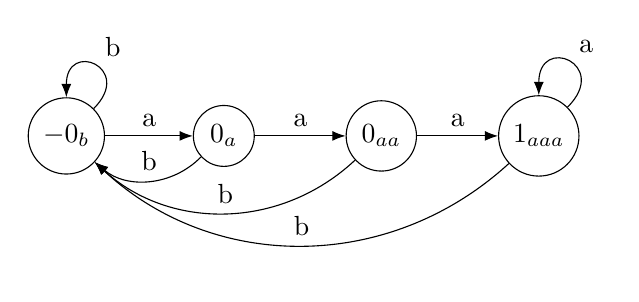
\begin{tikzpicture}[node distance={20mm}, main/.style = {draw, circle}]
            \node[main] (X) {$-0_b$};
            \node[main] (Y) [right of=X] {$0_a$};
            \node[main] (Z) [right of=Y] {$0_{aa}$};
            \node[main] (U) [right of=Z] {$1_{aaa}$};

            \path[-Latex] (X) edge node[above] {a} (Y);
            \path[-Latex] (Y) edge node[above] {a} (Z);
            \path[-Latex] (Z) edge node[above] {a} (U);

            \path[-Latex] (U) edge [out=45,in=90,looseness=5] node[above right] {a} (U);
            \path[-Latex] (X) edge [out=45,in=90,looseness=5] node[above right] {b} (X);
            \path[-Latex, bend left=15mm] (Y) edge node[above] {b} (X);
            \path[-Latex, bend left=15mm] (Z) edge node[above] {b} (X);
            \path[-Latex, bend left=15mm] (U) edge node[above] {b} (X);
        \end{tikzpicture}

    \item Construct a Mealy Machine that generates a 1 each time an
        occurrence of the pattern ``aaa" is detected in an input string; 0's may
        be generated at other times. Please note: ``aaaabaaa" contains THREE
        occurrences of ``aaa". \\
        \textbf{ANSWER:} \\
        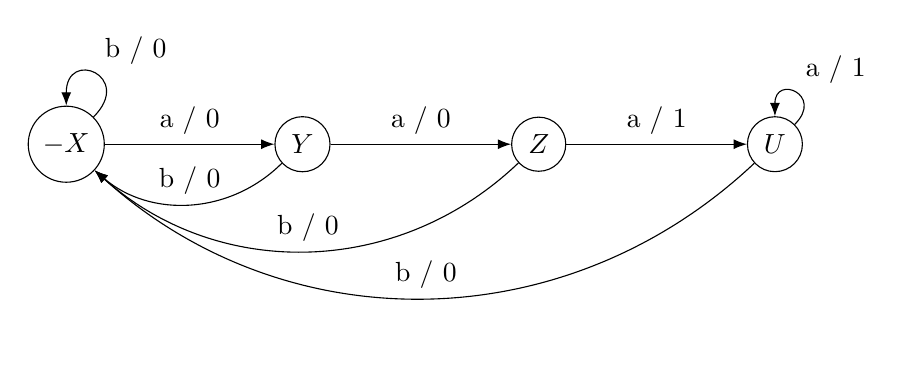
\begin{tikzpicture}[node distance={30mm}, main/.style = {draw, circle}]
            \node[main] (X) {$-X$};
            \node[main] (Y) [right of=X] {$Y$};
            \node[main] (Z) [right of=Y] {$Z$};
            \node[main] (U) [right of=Z] {$U$};

            \path[-Latex] (X) edge node[above] {a / 0} (Y);
            \path[-Latex] (Y) edge node[above] {a / 0} (Z);
            \path[-Latex] (Z) edge node[above] {a / 1} (U);

            \path[-Latex] (U) edge [out=45,in=90,looseness=5] node[above right] {a / 1} (U);
            \path[-Latex] (X) edge [out=45,in=90,looseness=5] node[above right] {b / 0} (X);
            \path[-Latex, bend left=15mm] (Y) edge node[above] {b / 0} (X);
            \path[-Latex, bend left=15mm] (Z) edge node[above] {b / 0} (X);
            \path[-Latex, bend left=15mm] (U) edge node[above] {b / 0} (X);
        \end{tikzpicture}

    \item Apply the constructive algorithm for \underline{complement} to FA$_1$
        given on slide 18 of Lecture 8. \\
        \textbf{ANSWER:} \\
        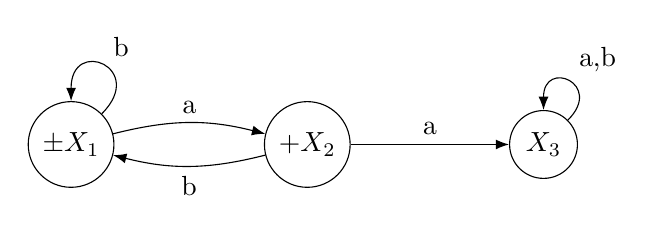
\begin{tikzpicture}[node distance={30mm}, main/.style = {draw, circle}]
            \node[main] (1) {$\pm X_1$};
            \node[main] (2) [right of=1] {$+X_2$};
            \node[main] (3) [right of=2] {$X_3$};

            \path[-Latex] (1) edge [out=45,in=90,looseness=5] node[above right] {b} (1);

            \path[-Latex, bend left=5mm] (1) edge node[above] {a} (2);
            \path[-Latex, bend left=5mm] (2) edge node[below] {b} (1);

            \path[-Latex] (2) edge node[above] {a} (3);

            \path[-Latex] (3) edge [out=45,in=90,looseness=5] node[above right] {a,b} (3);
        \end{tikzpicture}

    \item Apply the constructive algorithm for \underline{intersection} to
        the finite automata given on slide 7 of lecture 7 (our
        \underline{previous} lecture). Is there anything unusual about the FA
        the algorithm generates? If so, explain. \\
        \textbf{ANSWER:} \\
        \textbf{Step 1}: Create the starting state, $X_1Y_1$ \\
        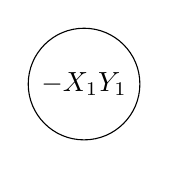
\begin{tikzpicture}[node distance={30mm}, main/.style = {draw, circle}]
            \node[main] (X1Y1) {$-X_1Y_1$};
        \end{tikzpicture}

        \textbf{Step 2}: Follow the paths for a and b from $X_1Y_1$, creating
        two new states, $X_2Y_1$ and $X_1Y_2$. \\
        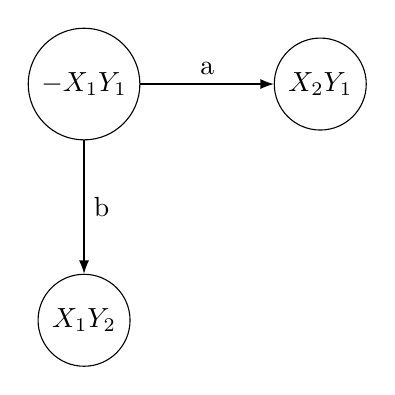
\begin{tikzpicture}[node distance={30mm}, main/.style = {draw, circle}]
            \node[main] (X1Y1) {$-X_1Y_1$};

            \node[main] (X2Y1) [right of=X1Y1] {$X_2Y_1$};
            \node[main] (X1Y2) [below of=X1Y1] {$X_1Y_2$};

            \path[-Latex] (X1Y1) edge node[above] {a} (X2Y1);
            \path[-Latex] (X1Y1) edge node[right] {b} (X1Y2);
        \end{tikzpicture}

        \textbf{Step 3}: Follow the paths for a and b from $X_1Y_2$, linking to
        $X_2Y_1$ and looping. \\
        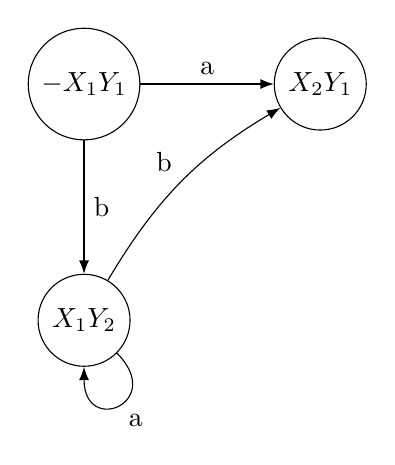
\begin{tikzpicture}[node distance={30mm}, main/.style = {draw, circle}]
            \node[main] (X1Y1) {$-X_1Y_1$};

            \node[main] (X2Y1) [right of=X1Y1] {$X_2Y_1$};
            \node[main] (X1Y2) [below of=X1Y1] {$X_1Y_2$};

            \path[-Latex] (X1Y1) edge node[above] {a} (X2Y1);
            \path[-Latex] (X1Y1) edge node[right] {b} (X1Y2);

            \path[-Latex, bend left=5mm] (X1Y2) edge node[above left] {b} (X2Y1);
            \path[-Latex] (X1Y2) edge [out=-45,in=-90,looseness=5] node[below right] {a} (X1Y2);
        \end{tikzpicture}

        \textbf{Step 4}: Follow the paths for a and b from $X_2Y_1$, linking to
        $X_1Y_2$ and looping. \\
        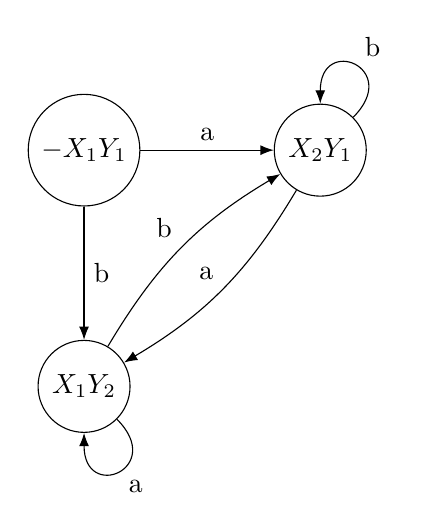
\begin{tikzpicture}[node distance={30mm}, main/.style = {draw, circle}]
            \node[main] (X1Y1) {$-X_1Y_1$};

            \node[main] (X2Y1) [right of=X1Y1] {$X_2Y_1$};
            \node[main] (X1Y2) [below of=X1Y1] {$X_1Y_2$};

            \path[-Latex] (X1Y1) edge node[above] {a} (X2Y1);
            \path[-Latex] (X1Y1) edge node[right] {b} (X1Y2);

            \path[-Latex, bend left=5mm] (X1Y2) edge node[above left] {b} (X2Y1);
            \path[-Latex] (X1Y2) edge [out=-45,in=-90,looseness=5] node[below right] {a} (X1Y2);

            \path[-Latex, bend left=5mm] (X2Y1) edge node[above left] {a} (X1Y2);
            \path[-Latex] (X2Y1) edge [out=45,in=90,looseness=5] node[above right] {b} (X2Y1);
        \end{tikzpicture}
\end{enumerate}

\end{document}
